\documentclass[border=0]{standalone}
\usepackage{tikz}
\usetikzlibrary{arrows,calc,positioning}
\renewcommand\rmdefault{\sfdefault}
% define simple color names for esa colors and a highlight
\definecolor{esa}{RGB}{10,156,215}
\def\esacolorfactor{20}
\colorlet{esa0}{esa!90!white}
\colorlet{esa1}{black!\esacolorfactor!esa0}
\colorlet{esa2}{black!\esacolorfactor!esa1}
\colorlet{esa3}{black!\esacolorfactor!esa2}
\colorlet{esa4}{black!\esacolorfactor!esa3}
\colorlet{esa5}{black!\esacolorfactor!esa4}
\definecolor{highlight}{RGB}{189,27,27}



\begin{document}
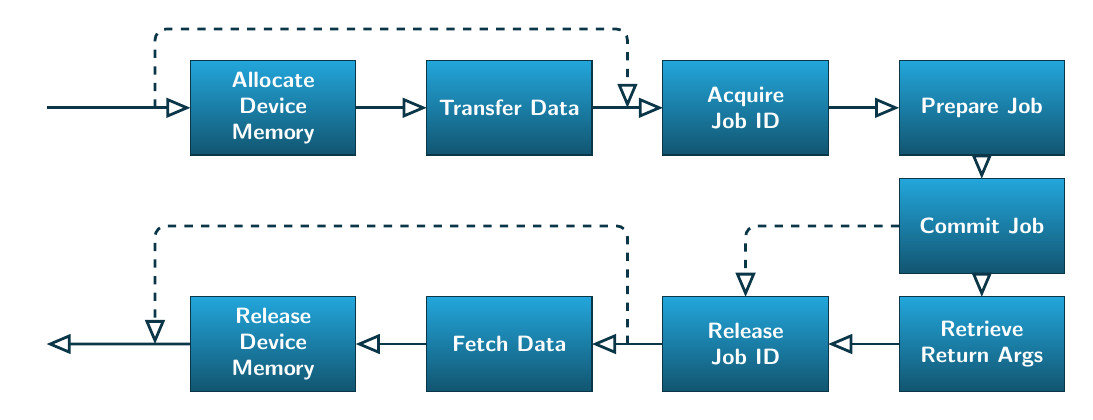
\begin{tikzpicture}[
    tapasco api step/.style={align=center, text width=1.8cm, font=\sffamily\footnotesize\bfseries\color{white}, minimum width=2.1cm, draw=esa5, top color=esa0, bottom color=esa3, outer sep=0pt, minimum height=1.2cm},
    chain/.style={draw=esa5, thick, ->, >= open triangle 45, line width=1pt, rounded corners},
    branch/.style={chain, dashed}
  ]
  \node (start) {};
  \begin{scope}[every node/.style={tapasco api step}, node distance=3cm]
  \node [right of=start] (alloc) {Allocate Device Memory};
  \node [right of=alloc] (transfer) {Transfer Data};
  \node [right of=transfer] (acjob) {Acquire Job ID};
  \node [right of=acjob] (jobpr) {Prepare Job};
  \node [below of=jobpr, node distance=1.5cm] (launch) {Commit Job};
  \node [below of=launch, node distance=1.5cm] (return) {Retrieve Return Args};
  \node [left of=return] (rljob) {Release Job ID};
  \node [left of=rljob] (fetch) {Fetch Data};
  \node [left of=fetch] (relmem) {Release Device Memory};
  \end{scope}
  \node [below of=start, node distance=3cm] (end) {};

  \begin{scope}[every path/.style={chain}]
  \path (start) -- (alloc);
  \path [branch] ($(start)!.5!(alloc)$) -- ++(0,1cm) -| ($(transfer)!.5!(acjob)$);
  \path (alloc) -- (transfer);
  \path (transfer) -- (acjob);
  \path (acjob) -- (jobpr);
  \path (jobpr) -- (launch);
  \path (launch) -- (return);
  \path [branch] (launch) -| (rljob);
  \path (return) -- (rljob);
  \path (rljob) -- (fetch);
  \path [branch] ($(rljob)!.5!(fetch)$) -- ++(0,1.5cm) -| ($(relmem)!.5!(end)$);
  \path (fetch) -- (relmem);
  \path (relmem) -- (end);
  \end{scope}
\end{tikzpicture}
\end{document}
